\problemname{Deiling}

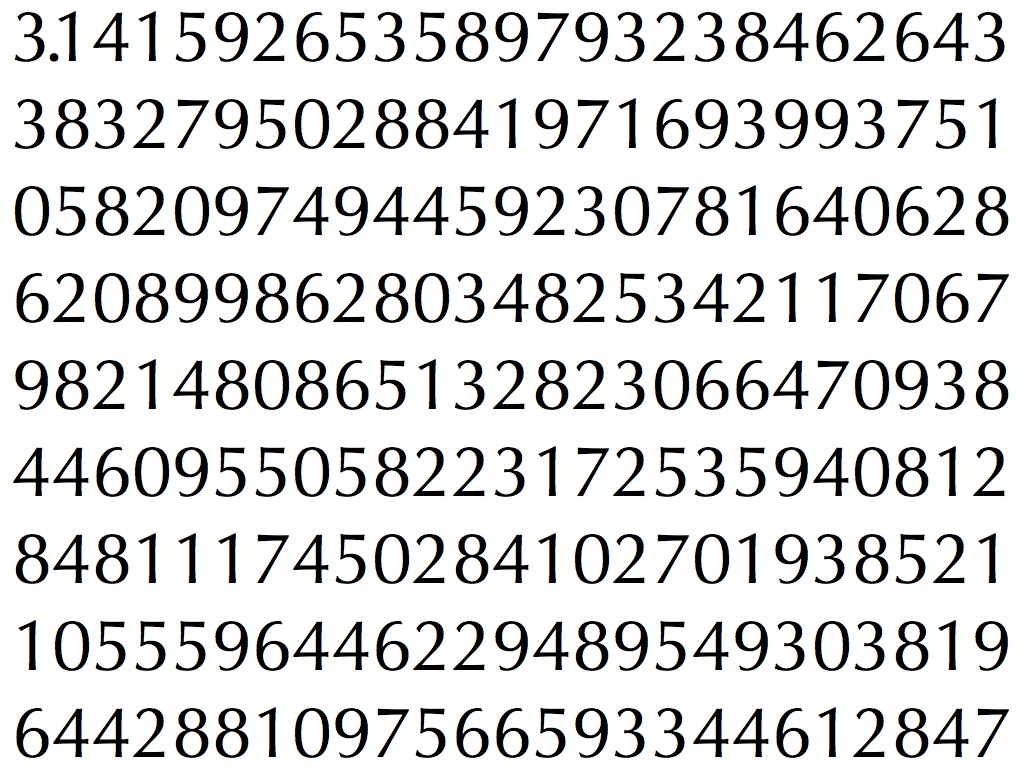
\includegraphics[scale=0.4]{pi.jpg}

Deiling er mikilvæg grunnaðgerð í stærðfræði og kemur bókstaflega allstaðar
fyrir. Einn skemmtilegur eiginleiki deilingar er að deiling tveggja heiltalna,
sem geta verið mjög litlar, getur gefið svar sem er rauntala með óendanlega
marga aukastafi. Ef við deilum 823 með 70, þá fáum við rauntöluna

$$11.7571428571428571428571428571428\ldots$$

Þessi tala hefur óendanlega marga aukastafi, en takið þó eftir því að aukastafirnir
eru í raun og veru bara tölustafurinn 7, og svo talnarunan 571428 endurtekin
aftur og aftur. Við getum táknað þessa tölu á forminu 11.7(571428), þar sem
talnarunan innan sviganna er talnarunan sem er endurtekin.

Þegar deiling er framkvæmd á tvær heiltölur, þá mun svarið vera rauntala.
Þrennt getur gerst þegar horft er á aukastafi tölunnar:

- talan hefur engan aukastaf (t.d. $8/4 = 2$)
- talan hefur endanlega marga aukastafi (t.d. $3/5 = 0.6$)
- talan hefur óendanlega marga aukastafi (t.d. $1/9 = 0.(1)$)

Ef talan hefur óendanlega marga aukastafi, þá munu aukastafirnir alltaf enda
með því að vera endurtekning á sömu talnarununni (eins og gerðist að ofan).

Inntakið samanstendur af tveimur heiltölum $0 \leq a \leq 100000$, $1 \leq b \leq 1000$ aðskildum með bili. Úttak
inniheldur eina línu sem inniheldur rauntöluna sem fæst með því að deila $a$ með
$b$. Ef rauntalan hefur óendanlega marga aukastafi á að skrifa hana á forminu sem
sýnt er að ofan.
